\chapter{Modelling} \label{chapter:4}

\section{Logistic Regression Results}

For the modelling, the data was split into train and test sets with proportions 0.7 and 0.3 respectively. The bad rate was maintained in each data at 17\% to ensure fairness and the variables were converted to their woe values for their respective bin from tables  (\ref{woe_1}) \& (\ref{woe_2}). Once split, the train data was passed through a glm model with logit link, for this the python package statsmodels was used \parencite{statsmodels}. Three models were created, first, seen in Table (\ref{table:results_1}), was the base model with every variable included with no changes. Looking at the results table we can see that the majority of variables are highly significant with p-values less than 0.001. Mortdue is deemed the most insignificant, most likely due to its high correlation with VALUE and as such the variance it explains is already captured by VALUE. This is confirmed if we run the model again with VALUE dropped, seen in Table (\ref{table:results_val_dropped}). The p-value for MORTDUE is now 0.0005. \\

For the second model we looked at applying log transformations to the variables which had a heavy right skew, LOAN, MORTDUE, VALUE and YOJ to try to improve their p-values. These values were then passed through the woe binning and the values converted. The IV of LOAN and YOJ improved by 0.01 and 0.03 respectively whilst MORTDUE and VALUE's IV decreased, based on this, only the log transformations of LOAN and YOJ were kept and used for the second model. The results for the second model can be seen in Table (\ref{table:results_2}). \\

Finally, a third model was made from dropping variables with high p-values, these were MORTDUE and REASON. The results are displayed in Table (\ref{table:results_3}). All the remaining variables have a p-value of less than 0.0001. Every coefficient is positive, implying that an increase in all variables increase in the probability of BAD, which from initial observation shouldn't be right. Looking back on Section (\ref{sec:variables}) we have some assumptions of large values decreasing the probability of BAD such as CLAGE and YOJ. The reason for this is a result of the WOE methods, changing the values of our binned variables to their respective WOE value seen in Tables (\ref{woe_1}) \& (\ref{woe_2}). Higher values of CLAGE have negative values, for example values of CLAGE between 180 and 240 have a woe value of -0.47. So in reality, a CLAGE value in this range would have the effect of decreasing the probability of BAD. \\

\begin{table}[H]
\renewcommand{\arraystretch}{1.25}
\begin{center}
\begin{tabular}{llll}
\hline
Model:              & GLM              & AIC:            & 2514.3936    \\
Link Function:      & logit            & BIC:            & -25781.2585  \\
Dependent Variable: & BAD              & Log-Likelihood: & -1245.2      \\
\hline
\end{tabular}
\end{center}
\begin{center}
\begin{tabular}{lrrrrrr}
\hline
             &  Coef.  & Std.Err. &    z     & P$> |$z$|$ &  [0.025 &  0.975]  \\
\hline
\hline
const        & -1.5770 &   0.0539 & -29.2635 &      0.0000 & -1.6826 & -1.4714  \\
DELINQ\_woe  &  1.0403 &   0.0790 &  13.1746 &      0.0000 &  0.8855 &  1.1951  \\
CLAGE\_woe   &  0.9281 &   0.1005 &   9.2313 &      0.0000 &  0.7311 &  1.1252  \\
NINQ\_woe    &  1.0073 &   0.1533 &   6.5722 &      0.0000 &  0.7069 &  1.3077  \\
MORTDUE\_woe & -0.1110 &   0.2344 &  -0.4737 &      0.6357 & -0.5705 &  0.3484  \\
CLNO\_woe    &  0.8184 &   0.1343 &   6.0959 &      0.0000 &  0.5553 &  1.0816  \\
LOAN\_woe    &  0.8540 &   0.1018 &   8.3890 &      0.0000 &  0.6545 &  1.0535  \\
REASON\_woe  & -0.4899 &   0.3985 &  -1.2295 &      0.2189 & -1.2709 &  0.2910  \\
JOB\_woe     &  0.8730 &   0.1629 &   5.3592 &      0.0000 &  0.5537 &  1.1923  \\
VALUE\_woe   &  0.8503 &   0.1535 &   5.5400 &      0.0000 &  0.5495 &  1.1512  \\
DEROG\_woe   &  0.7714 &   0.1046 &   7.3725 &      0.0000 &  0.5663 &  0.9764  \\
YOJ\_woe     &  0.8313 &   0.1992 &   4.1740 &      0.0000 &  0.4410 &  1.2217  \\
\hline
\end{tabular}
\end{center}
\caption{Results: Model 1 \label{table:results_1}}
\end{table}

\begin{table}[H]
\renewcommand{\arraystretch}{1.25}
\begin{center}
\begin{tabular}{llll}
\hline
Model:              & GLM              & AIC:            & 2494.3355    \\
Link Function:      & logit            & BIC:            & -25813.6256  \\
Dependent Variable: & BAD              & Log-Likelihood: & -1237.2      \\
\hline
\end{tabular}
\end{center}
\begin{center}
\begin{tabular}{lrrrrrr}
\hline
            &  Coef.  & Std.Err. &    z     & P$> |$z$|$ &  [0.025 &  0.975]  \\
\hline
\hline
const       & -1.5749 &   0.0540 & -29.1591 &      0.0000 & -1.6808 & -1.4691  \\
DELINQ\_woe &  1.0369 &   0.0791 &  13.1031 &      0.0000 &  0.8818 &  1.1920  \\
CLAGE\_woe  &  0.9499 &   0.1007 &   9.4281 &      0.0000 &  0.7524 &  1.1473  \\
NINQ\_woe   &  1.0102 &   0.1525 &   6.6229 &      0.0000 &  0.7112 &  1.3091  \\
CLNO\_woe   &  0.7860 &   0.1331 &   5.9031 &      0.0000 &  0.5250 &  1.0469  \\
LOAN\_woe   &  0.8042 &   0.0934 &   8.6116 &      0.0000 &  0.6212 &  0.9872  \\
JOB\_woe    &  0.8508 &   0.1630 &   5.2195 &      0.0000 &  0.5313 &  1.1703  \\
VALUE\_woe  &  0.7937 &   0.1230 &   6.4517 &      0.0000 &  0.5526 &  1.0348  \\
DEROG\_woe  &  0.7840 &   0.1048 &   7.4802 &      0.0000 &  0.5785 &  0.9894  \\
YOJ\_woe    &  0.8988 &   0.1660 &   5.4148 &      0.0000 &  0.5735 &  1.2241  \\
\hline
\end{tabular}
\end{center}
\caption{Results: Model 3 \label{table:results_3}}
\end{table}

The performance of each model is shown and compared in Table (\ref{perf_eval}). It can be seen from this table that based on the performance evaulation mentioned in Section (\ref{sec:perf_eval}). Model 2 and 3 appear to out perform Model 1. But, when comparing the Model 2 to 3, the difference between performance indicators becomes smaller. Model 3 improves on every performance indicator but only by a small margin when compared to the change from Model 1 to Model 2. Based on Table (\ref{perf_eval}) either Model 2 or 3 would be an appropriate choice but we will go with Model 3. Even though the AIC of model 3 is smaller, this is still only a difference of 1.08. Where as the log-likelihood has a difference of 1.5 with model 2 performing better. This implies that Model 3 is only considered better when evaluting the AIC because of the removal of two variables and being a smaller model. Despite this, Model 3 still out performs Model 2 in the other 3, it has a higher K-S Statisitc, meaning it's best point of seperation is stronger than Model 2, a higher GINI coefficient implies it has a higher discriminatory power and the higher divergence value tells us that the scorecard has a stronger seperation of the distribution of goods and bads. \\

\begin{table}[H]
\begin{center}
\renewcommand{\arraystretch}{1.25}
\begin{tabular}{lcccc}
\toprule
Model & AIC & KS & GINI & Divergence \\
Model 1 (Default) & 2514.39 & 0.4581 & 0.5956 & 1.3802  \\
Model 2 (Log transformations) & 2495.42 & 0.4814 & 0.6078 & 1.4439  \\
Model 3 (REASON and MORTDUE dropped) & 2494.34 & 0.4822 & 0.6116 & 1.4568 \\
\bottomrule
\end{tabular}
\caption{Performance Evaluation Results On Test \label{perf_eval}}
\end{center}
\end{table}

\section{Scorecard Building}

With the model selected we then needed to turn the logistic regression results into a readable scorecard. To do this, we again used the scorcard package in python \parencite{statsmodels} and used the function \textit{scorecard(bins, model, xcolumns, point0, odds0, pdo)}. The function takes the woe bins in Tables (\ref{woe_1}) \& (\ref{woe_2}) and the logistic coefficients from Table (\ref{table:results_3}) and develops a points system for each variable and their bins. The function uses Equation (\ref{eq:scorecard}) to calculate each bin's point value.\\

\begin{equation}\label{eq:scorecard}
Score_{i,j} = -\dfrac{pdo}{\ln(2)} \cdot WOE_{j} \cdot \beta_{i}
\end{equation}

where i is the ith variable, j is the jth bin of the ith variable and pdo is the points to double odds which for this project is assigned to 50. \\

The full table of scores for each bin can be found in the Appendix in Table (\ref{table:scorecard_points}). The total score of an applicant would then be the sum of these points for the respective bin the applicant falls into for each variable. This is demonstrated by the example of two applicants in Table (\ref{table:app_example}). We can see applicant 1 an ideal candidate, is requesting a large loan against a large equity. Their job is within the office category which has the lowest bad rate and no dergoatory marks or delinquencies against them. The scorecard assigns a score of 872 for this applicant. Applicant 2 on the other hand does not appear from inital obsevation, appealing to a lender. A relatively low loan against an average equity results in a lower potential profit against a weaker collateral. The applicant is self employeed, one of the riskier job categories and they also have a delinquent credit line. The scorecard assigned a score of 610 to this applicant. \\ 

\begin{table}[H]
\begin{center}
\begin{tabular}{lrrrr}
\toprule
& \multicolumn{2}{c}{Applicant 1} & \multicolumn{2}{c}{Applicant 2} \\
Variable & Observation & Score & Observation & Score \\
\midrule
BASE & & 701 & & 701 \\ 
LOAN & 9.93 & 27.0 & 8.51 & -89.0 \\
VALUE & 220886 & 44.0 & 82575 & 17.0 \\
JOB & Office & 30.0 & Self & -24.0 \\
YOJ & 2.639 & -2.0 & 2.08 & 14.0 \\
DEROG & 0 & 11.0 & 0 & 11.0 \\
DELINQ & 0 & 27.0 & 1 & -58.0 \\
CLAGE & 213.91 & 32.0 & 335.03 & 64.0\\
NINQ & 1 & -1.0 & 3 & -29.0 \\
CLNO & 32 & 3.0 & 42 & 3.0 \\
\midrule
Score &  & 872 &  & 610
\end{tabular}
\end{center}
\caption{Scorecard Applicant Example \label{table:app_example}}
\end{table}

In Figure (\ref{scorecard_plot}) the score of every applicant in the train and test data is plotted. The figure displays the distribution and bad probability for each set. You can see the distributions appear to follow the same trend but on the lower end seem to vary slightly, this is most likely due to the smaller sample size of clients that have been scored in this range. Going back to our two applicants we can take a look at what area they fall in. Applicant 1 is placed in the highest band and has a bad probability of less than 0.01, there would be no reason this applicant would not be approved for the loan based on our scorecard. Applicant 2 is placed into one of the lower bands with a bad rate around 0.35, wether this applicant would be accepted or reject would depend on where a lender choses their cut-off score to be. It could be possible that this applicant would land in their soft-cut off area and reviewed and accepted but what we do know is that based off this scorecard, applicant 2's chance of acceptance is relatively low. \\

The PSI value of our scorecard is 1.1\% indicating the two samples don't have a shift in population. In Figures (\ref{fig:sc_dist_train}) \& (\ref{fig:sc_dist_test}) we can also see a clear seperation of goods and bads within our scorecard with bads clearly on the lower end of the scorecard and goods on the upper. 

%\begin{figure}[!ht]
%	\centering
%	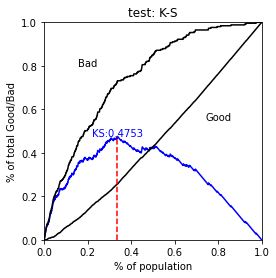
\includegraphics[scale=0.90]{figs/ks_plot.png}
%	\caption{KS Plot \label{ks_plot}}
%\end{figure}
%
%\begin{figure}[!ht]
%	\centering
%	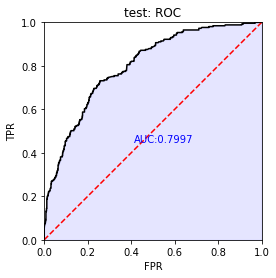
\includegraphics[scale=0.90]{figs/roc_plot.png}
%	\caption{ROC Plot \label{roc_plot}}
%\end{figure}

\begin{landscape}
\begin{figure}[!ht]
\begin{center}
	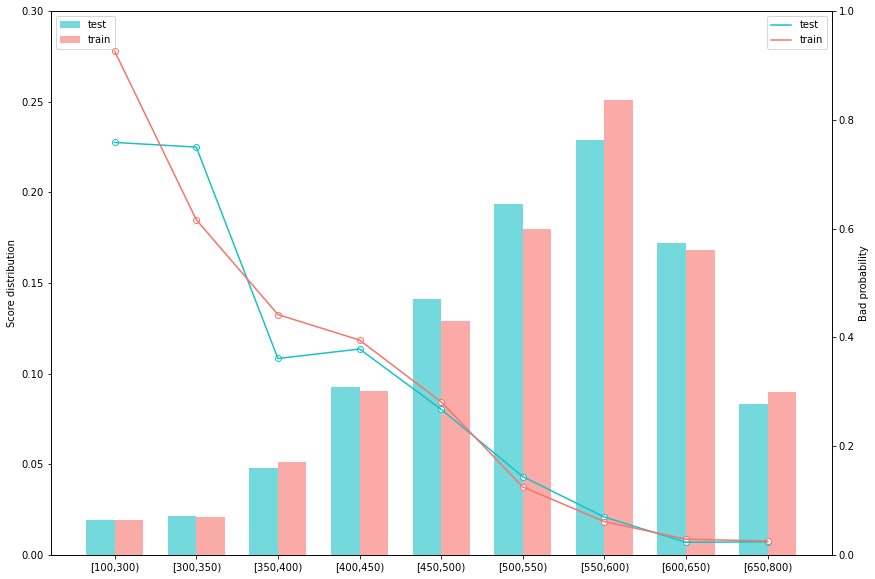
\includegraphics[scale=0.70]{figs/scorecard_plot.png}
	\caption{Scorecard Plot \label{scorecard_plot}}
\end{center}
\end{figure}
\end{landscape} 

\begin{figure}
\centering
  \centering
  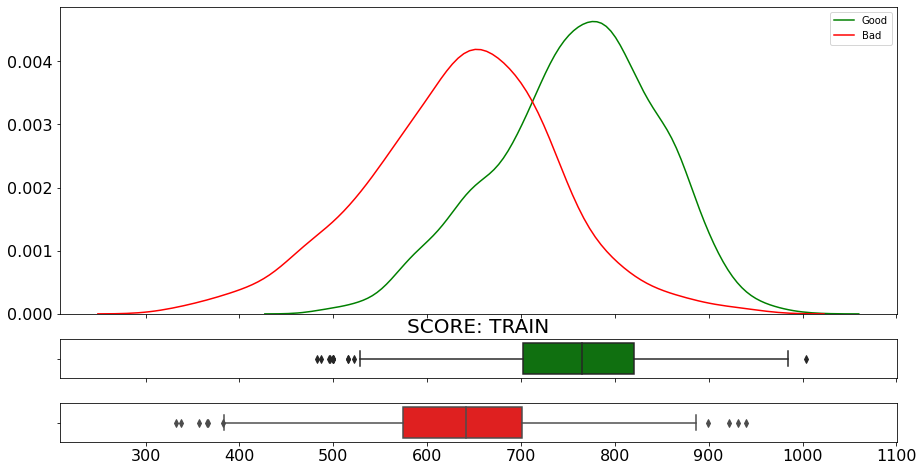
\includegraphics[width=0.9\linewidth]{figs/scorecard_dist_train.png}
  \caption{Scorecard Distribution for Train data}
  \label{fig:sc_dist_train}
\end{figure}

\begin{figure}
\centering
  \centering
  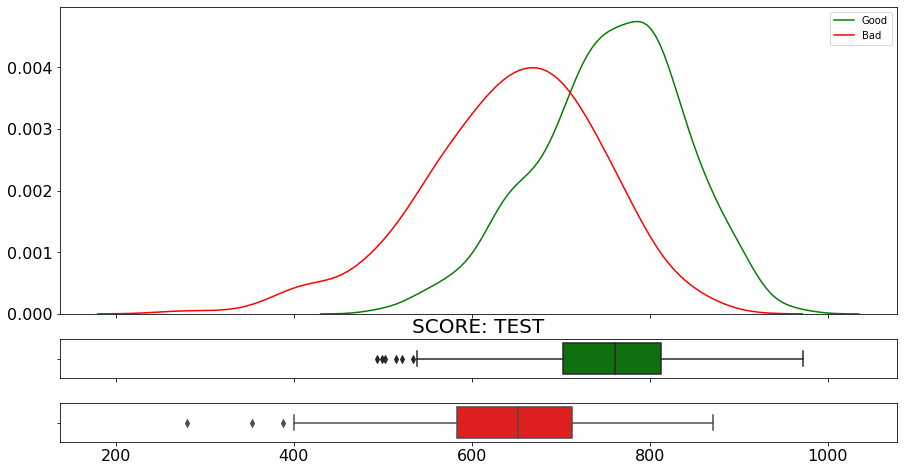
\includegraphics[width=0.9\linewidth]{figs/scorecard_dist_test.png}
  \caption{Scorecard Distribution for Test data}
  \label{fig:sc_dist_test}
\end{figure}
